\section{Purpose}

This Software Requirement Specification defines the functional and non-functional requirements for the Automated Shelf Monitoring System for Retail Stores.

\section{Functional Requirements}

\subsection{Shelf Image Capture}
\begin{itemize}
    \item The system must ingest shelf images from a single camera source at configurable intervals.
    \item We don't support scanning by "uploading" static images. Rather, it allows for capturing live feed at any instant manually, alongside the automated periodic frame captures.
\end{itemize}

\subsection{Product Occupancy Detection}
\begin{itemize}
    \item The system must detect whether each monitored shelf region is occupied or empty.
    \item The system must identify product SKUs for reconstructed stock analytics (e.g., beverages, snacks, personal care).
    \item The system must maintain a sliding history of occupancy status for each shelf region.
\end{itemize}

\subsection{Alert Generation}
\begin{itemize}
    \item The system must generate an alert when a shelf region transitions from occupied to empty.
    \item The system must provide an alert reason and the location of the empty region.
    \item The system must allow staff to mark alerts as resolved.
\end{itemize}

\subsection{User Interface}
\begin{itemize}
    \item The system must display the current shelf occupancy status in a simple dashboard.
    \item The system must show the last processed image and overlay detected empty regions.
    \item The system must list active alerts with timestamps and resolution status.
\end{itemize}

\section{Non-functional Requirements}

\subsection{Performance}
\begin{itemize}
    \item The system must process a captured shelf image within 5 seconds.
    \item The system must update the occupancy dashboard within 10 seconds of image capture.
\end{itemize}

\subsection{Accuracy}
\begin{itemize}
    \item The detection model must achieve at least 90\% precision for occupied vs.\ empty shelf regions.
    \item The system must correctly identify at least 85\% of selected product SKUs in evaluation data.
\end{itemize}

\subsection{Reliability}
\begin{itemize}
    \item The system must handle intermittent camera input loss and continue processing when the stream resumes.
    \item Alerts must remain available until staff explicitly acknowledges them.
\end{itemize}

\subsection{Usability}
\begin{itemize}
    \item The dashboard interface must be clear and accessible for retail staff without technical training.
    \item Alerts and occupancy status information must be understandable at a glance.
\end{itemize}

\section{Use Cases}

\subsection{Use Case 1: Monitor Shelf Status}

\textbf{Actor:} Store staff \\
\textbf{Trigger:} A new shelf image is captured.\\
\textbf{Precondition:} The camera feed is available.\\
\textbf{Postcondition:} The dashboard shows the updated occupancy status.

\subsection{Use Case 2: Receive Restocking Alert}

\textbf{Actor:} Store staff \\
\textbf{Trigger:} A shelf region is detected as empty.\\
\textbf{Precondition:} The occupancy detector has processed the latest image.\\
\textbf{Postcondition:} An alert appears in the alert list with location details.

\subsection{Use Case 3: Acknowledge Alert}

\textbf{Actor:} Store staff \\
\textbf{Trigger:} Staff reviews an active alert.\\
\textbf{Precondition:} The alert is active and unresolved.\\
\textbf{Postcondition:} The alert is marked resolved and archived.

\begin{figure}[H]
    \centering
    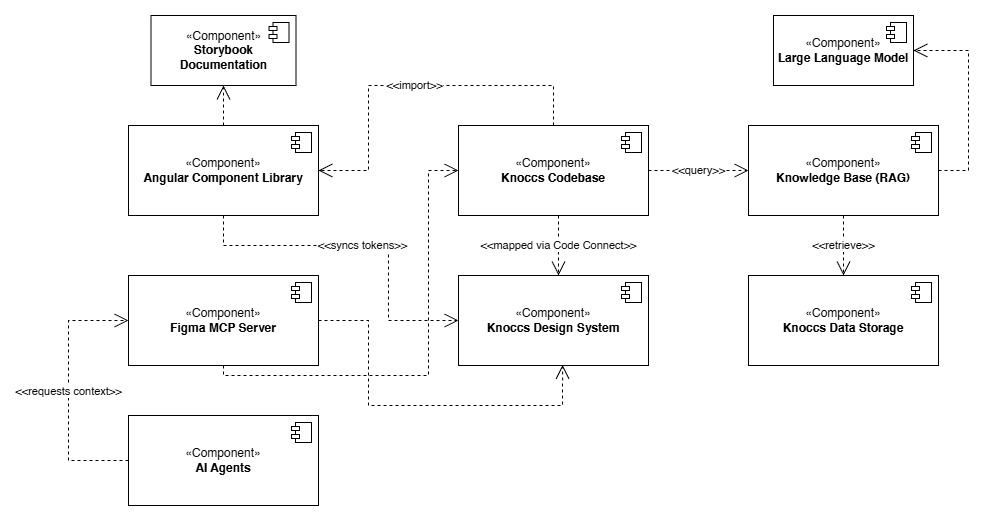
\includegraphics[width=0.8\textwidth]{figures/srs/Block Diagram.jpg}
    \caption{Use Case Diagram (Placeholder - to be added)}
    \label{fig:use-cases}
\end{figure}
